\documentclass[a4paper,oneside,11pt,english]{scrartcl} 

%% Preamble
\usepackage[onehalfspacing]{setspace}
\usepackage[nohyperlinks, printonlyused, withpage, smaller]{acronym}
\usepackage{graphicx}
\graphicspath{ {media/} }

\usepackage[hyphens]{url}
\urlstyle{same}

\usepackage[backend=biber, style=numeric, giveninits=true, bibencoding=utf8,sorting=none]{biblatex}
\addbibresource{bmc_article_covidPD.bib}
\DeclareNameAlias{author}{last-first}

%\usepackage[square,numbers,sort]{natbib}
%\bibliographystyle{abbrvnat}

\usepackage{subcaption}
\captionsetup[subfigure]{width=0.9\textwidth}

\usepackage{booktabs}
\usepackage{multirow}
\usepackage{makecell}
\usepackage{rotating}
\usepackage{longtable}

\begin{document}
	
\begin{titlepage}
	\noindent\Large{\textbf{Impact of the \textsc{Covid}-19 Pandemic on Perceived Access and Quality of Care in German People with Parkinson's Disease}}
	
	\subsection*{Authors:}
	Marlena van Munster$^{a}$, Marcel R. Prinz$^{a}$, David J. Pedrosa$^{a,b,*}$\\
		
	\noindent\small{$^{a}$ Department of Neurology, Philipps University Marburg, Baldingerstraße, 35043 Marburg, Germany}\\
	\small{$^{b}$ Centre of Mind, Brain and Behaviour, Philipps University Marburg, Hans Meerwein Straße 6, 35032 Marburg, Germany}\\

	\fontsize{7}{7}{$^{*}$ correspondence: Department of Neurology, Philipps University Marburg, Baldingerstraße, 35043 Marburg, Germany - david.pedrosa@staff.uni-marburg.de}´

	\vspace{2.5cm}
	\subsection*{Running title:}
	\textsc{COVID}-19 – Impact on Care Quality in Parkinson's disease\\
	
\end{titlepage}


\section*{Abstract}
\subsection*{Background}
Due to a heterogeneous clinical presentation, people with Parkinson´s disease (PwPD) develop different healthcare needs during their disease's course. Yet, the \textsc{Covid}-19 pandemic has disrupted the provision of some health resources, putting Pw\textsc{PD} at risk of inadequate care. Meanwhile, research on the social determinants of health (SDH) suggests an uneven burden among vulnerable populations.
\subsection*{Objective}
This study examined the influence of SDH on the perceived healthcare among PwPD during the pandemic in Germany.
\subsection*{Methods} 
All analyses relied on an anonymous online survey with a 49-item questionnaire. The aim of this survey was to describe access to health services before and during an early stage of the pandemic. To this end, a General Linear Model (GLM) was used to derive significant predictors and a stepwise regression aimed at summarising the main factors contributing to inadequate care.  
\subsection*{Results}
In total, 551 questionnaires were filled out showing that satisfaction for \textsc{PD}-related care decreased significantly during the pandemic (\textit{p} $<$ .001). Nevertheless, factors such as educational level, perceived expertise of healthcare providers, confidence in remote care, perceived ease of obtaining healthcare and the ability to access care prior to the pandemic, the density of neurologists within the area of living and the ability to overcome barriers were indicative of higher odds to perceive unmet needs during the pandemic (\textit{p} $<$ .05).
\subsection*{Conclusion}
The results unveil obstacles contributing to PwPD reduced access to healthcare during the \textsc{Covid}-19 pandemic. The findings may guide which societal and individual factors to address in a future in order to improve healthcare provision.
\subsection*{Keywords}
Parkinson's disease; \textsc{Covid}-19 pandemic; health care; impact; influence; Germany; iCARE-\textsc{PD}

\newpage

\section*{Introduction}
The \textsc{Covid}-19 pandemic presented modern societies with unprecedented challenges. The uncontrolled spread of a virus causing potentially fatal side effects despite intensive care and the resulting necessity to reduce everyday life afflicted societies economically and culturally. However, the impact on healthcare systems was particularly drastic. With rising incidences, public life around the world came to a standstill and access to public services, including health care, was disrupted \cite{nunez2021access, moynihan2021impact, world2020impact}. This disruption affected individuals in societies to varying degrees. The group of particularly affected subjects included those with chronic diseases \cite{sepulveda2020impact, kasar2021life, yogev2021covid, scheidt2021care}. This is not overly surprising in that people with chronic illnesses often belong to the high-risk group for a severe course of \textsc{Covid}-19, causing reluctance to attend medical facilities \cite{feral2020collateral}. Also, chronic conditions negatively affect individual psychosocial functioning \cite{demirtepe2022psychosocial}, often leaving affected persons in need of social, financial or physical support. People suffering from chronic diseases often necessitate continuous medical services outside of emergency departments and therefore appeared at high risk of undersupply during the pandemic \cite{scheidt2021care, nunez2021access, world2020impact}. 

The group of chronically-ill also includes people with Parkinson´s disease (Pw\textsc{PD}). Pw\textsc{PD} show a progressive condition characterized by motor but also non-motor symptoms. A plethora of different clinical signs may emerge during the disease's course, requiring continuous therapy adjustments and need assessments by healthcare professionals. Recent studies have unveiled the impact of the \textsc{Covid}-19 pandemic on people suffering from \textsc{PD} \cite{yogev2021covid, zipprich2020knowledge, frundt2022impact, richter2021analysis, brooks2021social}. However, it can hardly be assumed that all Pw\textsc{PD} were equally affected by the \textsc{Covid}-19 restrictions as other areas of public health research also indicate that health crises have very individual effects on health care access for vulnerable groups \cite{huijts2017prevalence, lowcock2012social, whocovidbrief}. 

In addition to individual health care needs, other determinants may be inferred that influence how severely care is restricted. In recent years, the concept of so-called social determinants of health (SDH) has emerged \cite{brown2020effect, world2010conceptual} which may pose an interesting concept to answer the question of what is relevant to maintain a high level of support and well-being individually but also on a societal level.

What may be considered relevant SDH is by no means universal. Rather, a context-specific consideration is required \cite{world2010conceptual}. For \textsc{PD}, Zaman et al. proposed a model summarising structural and individual factors potentially influencing patients' access to healthcare \cite{zaman2021barriers}. Structural SDH may on the one hand encompass barriers, that \textsc{PD}-patients meet on a system-level when accessing healthcare, such as a lack of care coordination, limited communication between healthcare providers, disparities in health services or the unavailability of specialised services \cite{zaman2021barriers}, etc. Otherwise, individual barriers influencing \textsc{PD}-patients' abilities to seek help or to engage with care providers, to reach important care services or to pay for them \cite{zaman2021barriers} may likewise be of great importance. Particularly people with \textsc{PD} often hinge on a good support network. 

To our knowledge, it has not yet been investigated how SDH may relate to the \textsc{Covid}-19 pandemic on access to healthcare in people with \textsc{PD}. Therefore, we examined the impact of a multitude of factors on this population with special emphasis on their access to healthcare during the pandemic in Germany. 

\newpage
%%%%%%%%%%%%%%%%
%% Methods    %%
%%%%%%%%%%%%%%%%

\section*{Methods}
\subsection*{Questionnaire}
Analyses relied on an anonymous survey carried out as part of the iCARE-\textsc{PD}-project (\url{https://icare-pd.ca/}). Within the scope of this project, a 49-items questionnaire was developed which aimed at characterising the access of Pw\textsc{PD} to healthcare services before and during the pandemic. The initial questions in English were translated to German and were structured in four sections: A) questions describing patients' health status in terms of \textsc{PD} but also of concomitant diseases, B) questions regarding experiences with healthcare services within twelve months before the pandemic, C) questions addressing experiences with healthcare services during the \textsc{Covid}-19 pandemic with special emphasis on telemedicine services, and, D) questions devoted to ascertaining demographic backgrounds of participants. There were single, multiple-choice questions or open-ended questions, some of which depended upon the specific answers to previous ones. A full version of the questionnaire is included in the supplementary data. 

The questionnaire was distributed nationwide using the members’ e-mail newsletter of the German Parkinson Association (Deutsche Parkinson Vereinigung e.V., dPV) between November 2020 to January 2021. The e-mail included a short invitation as well as a link to an online survey, which patients could access using a personal computer, a tablet or a smartphone. In Germany, SoSci Survey \cite{leiner2019sosci} served as a database for hosting the survey. Throughout the data input, the database was supervised and manually checked for plausibility. In addition to Germany, the iCARE-\textsc{PD} questionnaire was also shared with patient associations in Canada, Spain, Portugal and the Czech Republic with the respective translations. In this study, we limit ourselves to data collected from German patients. 

\subsection*{Additional data}
Within the last section of the survey, participants were asked to disclose the first three of five numbers of their German postal code, which allowed for regional data containment. We concatenated resulting data with publicly available population densities\footnote{\url{https://www.bbsr.bund.de/BBSR/DE/forschung/raumbeobachtung/Raumabgrenzungen/deutschland/regionen/Raumordnungsregionen/raumordnungsregionen-2017.xlsx?\_\_blob=publicationFile\&v=3}} and those for family doctors and neurologists\footnote{\url{https://gesundheitsdaten.kbv.de/cms/html/16402.php}}. Merging the available data with the maps for postal codes\footnote{\url{https://www.suche-postleitzahl.org/downloads}} resulted in regional distributions  (cf. Figure \ref{fig1:total}). Population densities and those for neurologists were stratified into five equal quantiles for further analyses. Moreover, the provided information of concomitant diseases (besides \textsc{PD}) was collated to a score -- the Elixhäuser Comorbitiy Score with its modification introduced by van Walraven et al. \cite{van2009modification} with higher values indicating more severe disease burden. Finally, all questions were assigned to barriers to accessing health services regarding \textsc{PD} as described by \cite{zaman2021barriers} (cf. Table \ref{tab3:matchingzaman} in the supplementary data).

\begin{figure}[h!]
\centering
\begin{subfigure}[b]{0.35\linewidth}
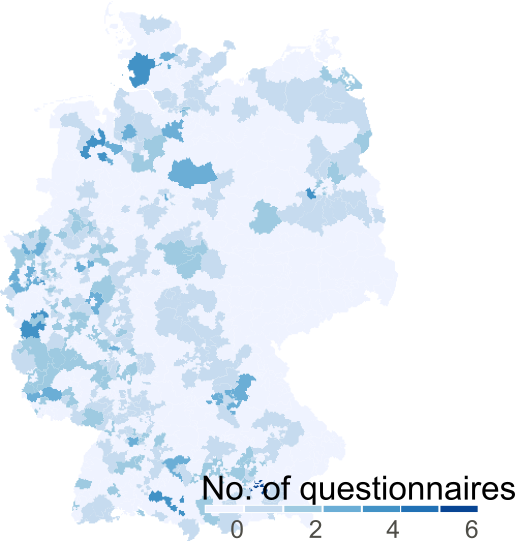
\includegraphics[width=.90\textwidth]{fig1a.questionnaires.v1.0.png}
\label{fig1:questionnaires}
\end{subfigure}%
\begin{subfigure}[b]{0.35\linewidth}
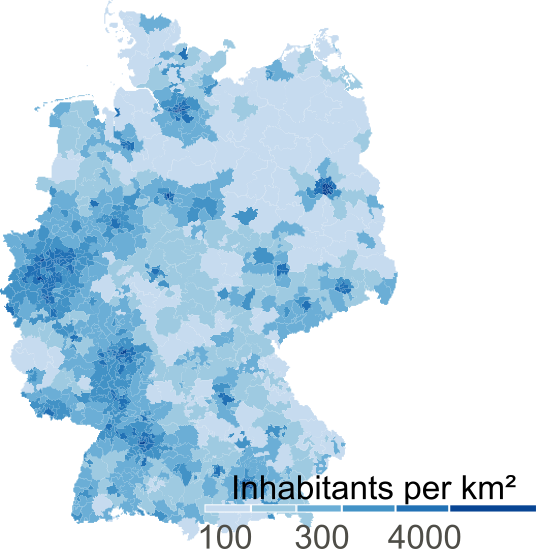
\includegraphics[width=.90\textwidth]{fig1b.population_density.1.0.png}
\label{fig1:population}
\end{subfigure}%
\begin{subfigure}[b]{0.35\linewidth}
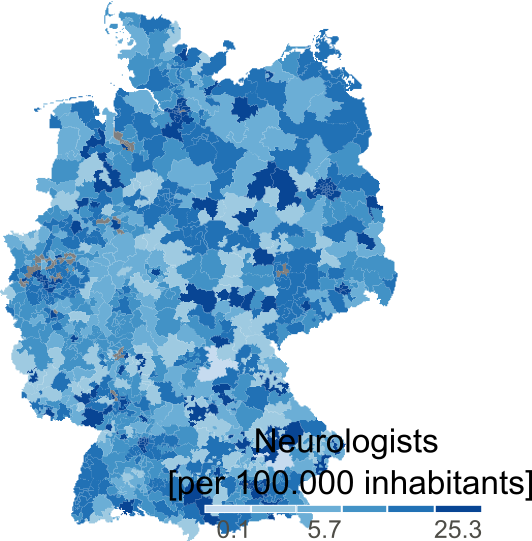
\includegraphics[width=.90\textwidth]{fig1c.neurologist_density.v1.0.png}
\label{fig1:neurologists}
\end{subfigure}%
\caption{Demographic data for Germany and additional regional data for the obtained questionnaires. A) Number of received questionnaires within our survey for the distinct three digit postal codes. B) Illustration of inhabitants per square kilometer for Germany. C) Density of neurologists in all parts of Germany according to the German Statutory Health Insurance Association (\textit{Kassenärztliche Bundesvereinigung})}
\label{fig1:total}
\end{figure}


\subsection*{Statistical analyses}
All analyses were conducted in R \cite{rcore}. After estimation of descriptive statistics, satisfaction with overall \textsc{PD}-related care was compared before and during the pandemic using a non-parametric \textit{sign-test} (rstatix package, \url{https://github.com/kassambara/rstatix/}). The two questions that were used were: 
\begin{itemize}
\item ``In the 12 months prior to the  \textsc{Covid}-19 pandemic, overall, how satisfied were you with the way healthcare services related to \textsc{PD} were provided?'' (B17) vs.
\item ``Since the beginning of the \textsc{Covid}-19 pandemic, overall, how satisfied are you with the way healthcare services related to \textsc{PD} are provided?'' (C6).
\end{itemize}

Furthermore, using a General Linear Model (\textsc{GLM}) we estimated the odds for worse satisfaction with \textsc{PD}-related care. After establishing the full model with a total of 32 predictors, we conducted a stepwise logistic regression in order to reduce the complexity leaving the most meaningful predictors for the question: ``Since the beginning of the \textsc{Covid}-19 pandemic, how often did you feel you needed healthcare for \textsc{PD} but did not receive it?'' (C4). For that purpose, first missing data were imputed by taking advantage of a multivariate imputation scheme using the \textsc{Mice}-package \cite{vanbuuren2011}. We thereby assumed data missing at random and used the Predictive Mean Matching Method. After missing data imputation, stepwise reduction using a \textsc{GLM} with Stepwise Feature Selection (\textit{glmStepAIC}) in both directions from the \textit{caret}-package \cite{kuhn2008} aimed at minimising the Akaike Information Criterion. For that, we first split all data into 80\% of training and 20\% of test data and performed the stepwise regression after centering and rescaling values and applying 10-fold cross-validation. The predictions of the two models were compared with the test data using Accuracy, Area Under the Curve (AUC) and LogLoss as metrics. All data for the analyses and all analyses can be followed under \url{https://github.com/dpedrosac/covidPD/}

\newpage
%%%%%%%%%%%%%%%%
%% Results %%
%%%%%%%%%%%%%%%%

\section*{Results}
In total, 551 questionnaires were filled out with 252 different postal codes from all 16 German regions (Bundesländer, cf. Figure~\ref{fig1:total}). 

Of all participants, 388 (70.4$\%$) returned a complete questionnaire (for demographics from parts A and D, cf. Table~\ref{table1}).

\begin{table}[h!]
	\caption{Demographics of subjects filling out questionnaire:}
	\label{table1}
	\begin{tabular}{p{10cm} c}
		\toprule
		&\textbf{Overall}\\ %\hline
		& \textbf{(n = 551)}\\ \hline

		Age (mean (SD)) & 66.76 (9.25) \\ \hline
		Gender = female (\%) &  148 (41.6)  \\ \hline
		Disease duration (\%) & \\ \hline
		\hspace{3mm} $<$2 years & 62 (13.1) \\ \hline
		\hspace{3mm} 2--5 years & 154 (32.6) \\ \hline
		\hspace{3mm} 5--10 years & 157 (33.2) \\ \hline
		\hspace{3mm} 10--15 years & 69 (14.6) \\ \hline
		\hspace{3mm} $>$15 years& 31 ( 6.6) \\ \hline
		Disease stage (\%)& \\ \hline
		\hspace{3mm} Hoehn \& Yahr I &  189 (40.3) \\ \hline
		\hspace{3mm} Hoehn \& Yahr II & 156 (33.3)  \\ \hline
		\hspace{3mm} Hoehn \& Yahr III  &   77 (16.4) \\ \hline
		\hspace{3mm} Hoehn \& Yahr IV  & 41 ( 8.7) \\ \hline
		\hspace{3mm} Hoehn \& Yahr V  &     6 ( 1.3) \\ \hline
		Education level according to ISCED (\%) & \\ \hline
		\hspace{3mm} primary education  & 20 ( 5.0) \\ \hline
		\hspace{3mm} secondary education  & 234 (58.4)\\ \hline
		\hspace{3mm} post secondary education  &   69 (17.2) \\ \hline
		\hspace{3mm} highest education level possible & 78 (19.5)  \\ \hline
		\hspace{3mm} \textsc{PD}Q-8 scores (mean (SD)) & 41.30 (14.23) \\ \hline
		Van-Walraven-Elixhauser Comorbidity Index (mean (SD) & 6.55 (1.95) \\ \hline
		\bottomrule
	\end{tabular}
\end{table}

Satisfaction for \textsc{PD}-related care significantly decreased during the pandemic. Hence, the \textit{sign-test} for the question: ```Overall, how satisfied are you with the way healthcare services related to \textsc{PD} are provided?'' indicated lower values during the pandemic (Mdn = 1) compared to before (Mdn = 3, \textit{p} = 10\textsuperscript{-73}). More than 90\% of all participants stating to be rather unsatisfied or very unsatisfied with their \textsc{PD}-related care during the pandemic (cf. Figure \ref{fig2:satisfaction}). 

\begin{figure}[h!]
\centering
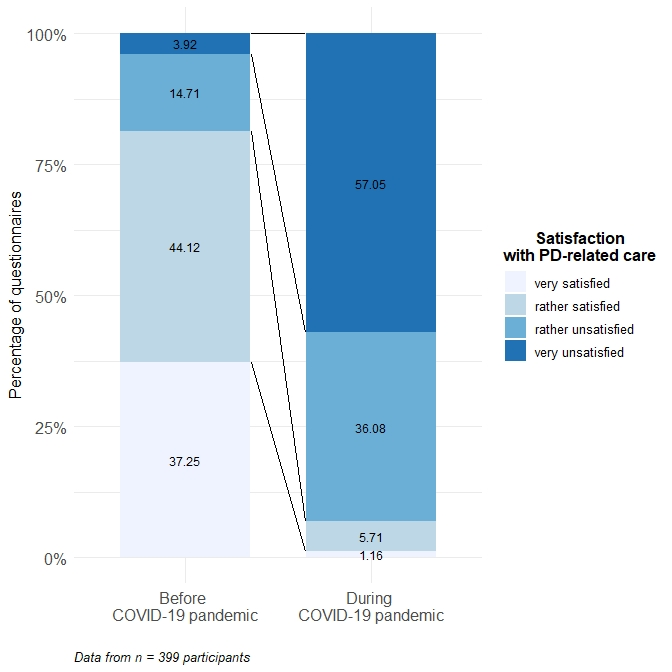
\includegraphics[width=.90\textwidth]{fig2.satisfaction.care.v1.0.jpeg}
\caption{B17 vs. C6 - Distribution of responses on the Satisfaction with PD-related care before and during the \textsc{Covid}-19 pandemic.}
\label{fig2:satisfaction}
\end{figure}

To ascertain underlying reasons for dramatic declines in satisfaction, logistic regressions on question C4 (``Since the beginning of the \textsc{Covid}-19 pandemic, how often did you feel you needed healthcare for \textsc{PD} but did not receive it?'') was performed, unveiling different factors which contributed to this perception of unmet needs during the pandemic (see Figure \ref{fig3:resultsOR1}). 

\begin{figure}[!h]
%Kann man die Grafik größer anzeigen und vielleicht sortieren?
%% DP: Wonach sortieren? Die Grafiken werden am Ende nicht eingefügt sondern als svg mitgeschickt, das Layout dürfen die übernehmen ;) 
\centering
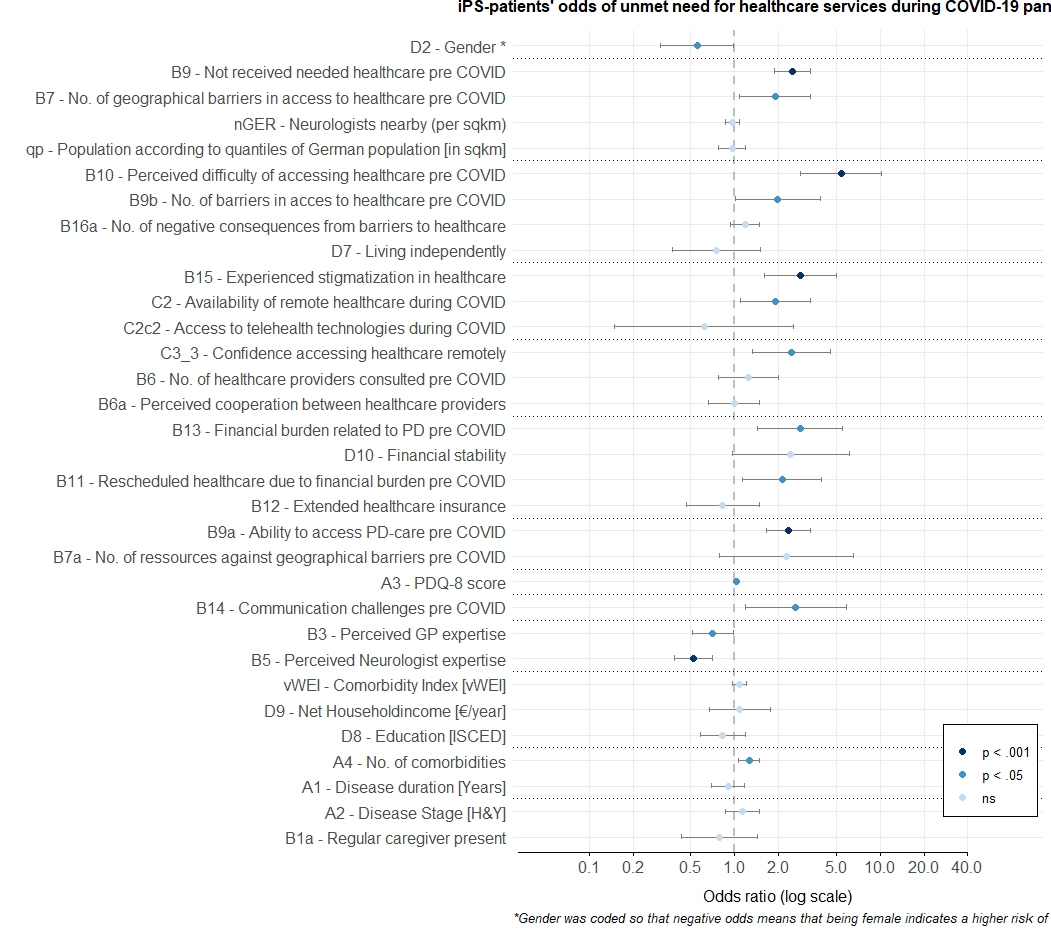
\includegraphics[width=\textwidth]{fig3.oddsratios.v1.0.jpeg}
\caption{Unadjusted Odds ratios according to the \textsc{GLM} for all 32 questions. Odds were determined so that higher values indicate affirmation to the question that healthcare was needed but this need remianed unmet during the \textsc{Covid}-19 pandemic. The dashed lines indicate the distinct domains according to Zaman et al. \cite{zaman2021barriers}, whereas significance is illustrated as color of the dot, with two distinct levels of significance. }
\label{fig3:resultsOR1}
\end{figure}



Thus, odds to affirm this question were highly significant (\textit{p} $<$ .001) for those patients inferring lower levels of competence for their neurologist, with a lower ability to access \textsc{PD}-care before the pandemic, for patients with higher degrees of stigmatisation in healthcare and for those who did not receive healthcare services before the pandemic. A significant contribution -- albeit lower with significance values \textit{p} $<$ .05 --  was encountered for Pw\textsc{PD} with increasing levels of comorbidity, with perceived lower expertise of the general practitioner, with higher quality of life scores retrospectively, for people with higher financial burden due to \textsc{PD} or who rescheduled healthcare due to financial burden before the pandemic. Finally, the lack of availability of remote healthcare during the pandemic and geographical or in general more numerous barriers in access to healthcare before the start of the pandemic were also indicative of higher odds to perceive unmet needs. For an illustration of significant predictors see Figure \ref{fig3:resultsOR1} and for the entire list of results cf. Table \ref{tab4:resultsall1} in the supplementary material. 

Starting with the entirety of 32 questions that might be predictors of affirming question ``C4'' (see above), using a two-way stepwise regression model these could be reduced to seven (cf. Table \ref{tab2:reduced_model}), namely: 
\begin{itemize}
	\item[--] educational level
	\item[--] perceived expertise of the general practitioner
	\item[--] confidence in the ability to access required health care services remotely
	\item[--] perceived ease of obtaining healthcare before the pandemic
	\item[--] perceived availability of specialist care before the pandemic
	\item[--] density of neurologists within the area of living
	\item[--] availability of structural support to overcome geographical barriers
\end{itemize}

\begin{table}[ht]
	\caption{Significant factors contibuting to unmet care needs during \textsc{Covid}-19 pandemic according to the reduced \textsc{GLM}:}
	\label{tab2:reduced_model}
	\centering
	\resizebox{\columnwidth}{!}{\begin{tabular}{l c c c c}
		\toprule   
		\textbf{Predictor}	& \textbf{Estimate}					& \textbf{SE} & \textbf{\textit{z}-value} & \textbf{\textit{p}} \\ \hline
		(Intercept) 											& -2.65  		& 0.29 	& -9.24 	& $<$.0001 \\ \hline
		Educational level (D8) 									& -0.73 		& 0.24 	& -3.01 	& 0.003 \\ \hline
		Perceived GP's expertise (B3) 							& 0.34 		& 0.17 	& 2.07 	& 0.038 \\ \hline
		Confidence in accessing necessary services remotely (C3) 	& 0.64 		& 0.22 	& 2.90 	& 0.004 \\ \hline
		Ease obtaining healthcare prior to the pandemic (B10)		& -0.47 		& 0.22 	& -2.15 	& 0.031 \\ \hline
		Ability to access care prior to the pandemic (B9)				& 0.41 		& 0.20 	& 2.07 	& 0.038 \\ \hline
		Density of Neurologists 									& 0.47 		& 0.21 	& 2.22 	& 0.027 \\ \hline
		Overcoming barriers (B7a)   								& -0.51 		& 0.22 	& -2.38 	& 0.017 \\ \hline
		\bottomrule
	\end{tabular}}
\end{table}	 

Markers for model comparison were indicative of similar performances in the ``full model'' with 32 predictors compared to the reduced one (cf. Figure \ref{fig4:comparison_models})

%Figure 4 hier einbinden

\newpage

%%%%%%%%%%%%%%%%
%% Discussion %%
%%%%%%%%%%%%%%%%

\section*{Discussion}
In this study, we sought to investigate factors contributing to insecurity and the feeling of not having received health services during the \textsc{Covid}-19 pandemic among German Pw\textsc{PD}. To the best of our knowledge, this is the first time that SDH were related to German \textsc{PD}-patients' perceived access to healthcare during this extraordinary crisis. With our study, we demonstrate that not all individuals were affected equally but that structural as well as individual determinants massively infer perceived access to healthcare. Viewing the pandemic through the focal lens of an ongoing demographic change in Western societies, our findings may render a deeper insight into how future care of Pw\textsc{PD} may be improved. 

It remains undisputed that the \textsc{Covid}-19 pandemic has been a defining event in recent years. At a relatively early stage and before the availability of vaccination provided some relief, our data reflect people's unbiased and acute concerns regarding their own healthcare. Interestingly, a good overall performance has been attested to the German healthcare system during the pandemic \cite{10665-341674}, which is transferable to Pw\textsc{PD} \cite{frundt2022impact}. However, a good testimony for a healthcare system should not be equated with an adequate range of services, especially when it comes to very specific needs of \textsc{PD}-patients. In the recent literature, care deficits on a structural level have been reported insinuating a rather partial insufficiency \cite{richter2019dynamics,van2020building, prell2020specialized, deuschl2016s3} of this heterogeneous population.

One of the major challenges physicians face in \textsc{PD} is its diverse manifestation. Multimodal therapeutic approaches could be a potential remedy \cite{richter2019dynamics}, yet limited availability of such services cause long journeys from people from some regions of Germany \cite{richter2019dynamics} as regionally coordinated care approaches for Pw\textsc{PD} remain rare \cite{van2020building}. Furthermore, staff providing specialised, structured and cooperative care services are lacking especially in outpatient care and in nursing homes \cite{prell2020specialized}, despite being advisable \cite{radder2020recommendations, deuschl2016s3}. Our results substantiate that structural challenges for individuals with \textsc{PD} reinforce perceived insecurity and a feeling of not obtaining the needed health care. The majority of predictors from the reduced model and eight predictors from the full model may be projected to system-level barriers as per Zaman et al.  

On the level of individual SDH, our data may also have some implications. We identified low educational attainment as a predictor for the perception of inadequate health care, which according to Zaman \cite{zaman2021barriers} relates to two dimensions: health literacy and self-efficacy. The former thereby inversely correlates with the ability to express healthcare needs \cite{davis2003variability, hurt2019barriers} -- another significant predictor in our data -- and with lower educational levels of Pw\textsc{PD} \cite{fleisher2016associations}. This is in good accordance with higher rates of hospitalisations and a higher caregiver burden \cite{fleisher2016associations} as well as higher disease severity \cite{fleisher2016associations} in Pw\textsc{PD} with lower health literacy. With regards to higher self-efficacy, this correlates the level of education\cite{lim2020factors} and, at the same time, with quality of life \cite{rostagni2022gratitude, lim2020factors}. Hence, our model suggests that Pw\textsc{PD} who have received more education and who present with higher quality of life scores show the greatest probability to absorb healthcare disruptions in healthcare. Our data advocates for greater attention to individuals with lower levels of education, but particularly those with a diminished quality of life from professionals involved in \textsc{PD}-patient care.

Unsurprisingly, Pw\textsc{PD} deemed the expertise of physicians, that is neurologists and general practitioners alike, important on the perception in adequate care. It is well-known that patients' trust in care professionals may foster healthcare utilization \cite{bainbridge2009challenges, shin2016initiation}. This warrants special emphasis since training appears at first glance accessible. The extent to which a trained Parkinson Nurse could facilitate special services and therefore complement medical expertise remains a question to be answered \cite{vanrole}. Yet, one might infer that they could catalyst tailored offerings such as legal or economic counselling. Hence, economic problems were highlighted in our results and are consistently cited as a reason for not seeking care services \cite{zaman2021barriers}, although being often neglected by physicians. Barring direct costs, e.g. those services spared from health insurance, many patients also claim indirect expenses like those resulting from the inability to work \cite{spottke2005cost}. This may gain importance with increases in the employment of women nowadays.  In general, however, a rather surprising result is that women are at higher risk of perceived undersupply. The reasons are unclear, but abundant literature indicates that women have fewer caregivers compared with their spouses \cite{dahodwala2018sex} especially, as they are less likely to receive care from their male partners \cite{zaman2021barriers}. A higher vulnerability to disruptions of healthcare because of the pandemic is therefore feasible and awaits future confirmation. In general, one might posit that to strengthen the resilience of \textsc{PD} health care, strategies are needed that recognize and address both structural and individual barriers in access to healthcare.

In addition to investments, reorganization and policy reforms on the structural level \cite{taylor2016leveraging, gottlieb2019social}, suitable assessments are also required to make the individual requirements of patients tangible for the treatment team \cite{friedman2018toward, gottlieb2019social}. One possible solution for subjects lacking access to healthcare services or who may not be able to ask for assistance due insufficient health literacy could be telehealth services. Telehealth services are effective means to facilitate access to care for Pw\textsc{PD} \cite{achey2014past, van2021moving}. In this questionnaire, we could corroborate these results as patients with access to these services before the pandemic reported a reduced likelyhood of unmet care needs. Nevertheless, some caution is advised when interpreting these findings as this cohort must be deemed rather technology-savy according to the nature of the questionnaire. Therefore, this process may not generalisable for all German patients \cite{eggers2020care}. Further investigations are warranted, e.g., on how to increase the confidence in telemedicine or how to overcome technological limitations such as high-speed internet availability. Another possible caveat to consider are putative unintended negative effects on health equity, so that Pw\textsc{PD} with low incomes or with other barriers to accessing technology could be left behind and thus underserved \cite{samuels2021digital}. 

\section*{General Limitations:}
Despite revealing problems patients encountered during the \textsc{Covid}-19 pandemic, the interpretation of our results requires some caution. Hence, it was an anonymous online survey, so that the representativeness for the German \textsc{PD} population is not warranted. As abovementioned, not only patients filling out the questionnaire may be highly selected from a major support group in Germany but especially the online tool also suggests that it is more likely to be filled out by tech-savvy patients. In this context, the mean age of almost 67 years was surprising, so that young-onset \textsc{\textsc{PD}}-patients cannot be inferred from this. Finally, a limitation is also the fact that there was no way to ascertain misdiagnosis or the correctness of data, so that these results await confirmation in observational studies with controlled demographics.

\section*{Conclusion}
In order to learn from the pandemic in the long term, difficulties in access to healthcare must be uncovered and addressed. The results of this analysis showed that the \textsc{Covid}-19 pandemic did not affect all \textsc{\textsc{PD}}-patients equally, but that people who experienced individual and structural barriers to accessing healthcare before the pandemic were more affected. Therefore, it is important to examine these determinants more closely and to address them in future-oriented, resilient healthcare models. Further investigations into the effect of individual and structural influences as by as Zaman et al. defined on measures of healthcare experiences should be object of further scrutiny. 

% \bibliographystyle{plainnat}
%\bibliography{bmc_article_covid\textsc{PD}}      
\printbibliography %[title={References}]

\newpage
\section*{Supplementary Material}
\begin{table}[!ht]
	\settowidth\rotheadsize{Personal-level}
	\caption{Matching of items in the questionnaire to the categories from the work of Zaman et al. \cite{zaman2021barriers}}
	\label{tab3:matchingzaman}
	\centering
	\begin{tabular}{l l l}
		\toprule 
		\textbf{Question from \textsc{Covid}-Survey}& \textbf{Representative for } \\
		\cmidrule{1-2}
		%& \textbf{Person-level Barriers} &	´\\ \hline
		1. A2, B1a, D7 & Autonomy  & \\
		\cmidrule{1-2}
		2. A1, A4, vWEI, B16a & Health Status &\\
		\cmidrule{1-2}
		3. D8 & Health Literacy & \\
		\cmidrule{1-2}
		4. B3, B5 & Health Belief & \multirow[t]{9}{*}{\rothead{\centering\textbf{Person-level Barriers}}} \\
		\cmidrule{1-2}
		5. B14 & Communication (personal) & \\
		\cmidrule{1-2}
		6. \textsc{PD}Q-8 & Self-efficacy &\\
		\cmidrule{1-2}
		7. B7a, B9a/b & Transportation &\\ 
		\cmidrule{1-2}
		8. B11, B12, B13, D9, D10 & Cost of care &\\
		\cmidrule{1-2}
		9. D2 & Other &\\ \hline
		%& \textbf{System-level Barriers} &\\ \hline
		10. NA & Difficulties of Diagnosis & \\
		\cmidrule{1-2}
		11. B6a & Coordination in care &\\
		\cmidrule{1-2}
		12. B15, C2c2 & Communication (system) & \multirow[t]{5}{*}{\rothead{\centering\textbf{System-level barriers}}}\\
		\cmidrule{1-2}
		13. B7, B9b, B10, C3\_3, nPop, nGer & Disparty in Health Services &\\
		\cmidrule{1-2}
		14. B6, B7a, B9, B9a, C2, C2c2 & Unavailability of Specalist Services & \\
		\bottomrule
	\end{tabular}
\end{table}

\newpage
\begin{longtable}[ht!]{|p{5.5cm} | p{3.5cm} | p{1cm} | l | l | p{1.5cm} |}
		\caption{Odds ratios for the distinct items of the questionnaire} 
		\label{tab4:resultsall1} \\ \hline
		\textbf{Factors} & \textbf{Domain} & \textbf{OR} & \textbf{CIlow} & \textbf{CIup} & \textbf{\textit{p}} \\ \hline
		\endhead
		A1 - Disease duration [Years] & Health Status & 0.9 & 0.69 & 1.16 & 0.419 \\ \hline
		A2 - Disease Stage [H\&Y] & Autonomy & 1.13 & 0.87 & 1.47 & 0.367 \\ \hline
		A4 - Presence of comorbidities & Health Status & 1.26 & 1.06 & 1.49 & 0.007 \\ \hline
		B1a - Regular caregiver present & Autonomy & 0.79 & 0.43 & 1.44 & 0.438 \\ \hline
		B3 - Perceived GP expertise & Health Belief & 0.71 & 0.51 & 0.98 & 0.038 \\ \hline
		B5 - Perceived Neurologist expertise & Health Belief & 0.52 & 0.39 & 0.7 & p $<$ .001 \\ \hline
		B6 - No. of healthcare providers consulted pre \textsc{Covid} & Unavailability of Specialitsts Services & 1.24 & 0.77 & 1.99 & 0.374 \\ \hline
		B6a - Perceived cooperation between healthcare providers & Coordination in Care & 0.99 & 0.66 & 1.49 & 0.975 \\ \hline
		B7 - Presence of geographical barriers in access to healthcare pre \textsc{Covid} & Disparty in Health Services & 1.9 & 1.08 & 3.33 & 0.026 \\ \hline
		B7a - No. of structural and transportation ressources against geographical barriers pre \textsc{Covid} & Unavailability of Specialists Services/ Transportation & 2.27 & 0.79 & 6.51 & 0.129 \\ \hline
		B9 - Not received needed healthcare pre \textsc{Covid} & Unavailability of Specialits Services & 2.5 & 1.88 & 3.32 & p $<$ .001 \\ \hline
		B9a - Availability of \textsc{PD}-specific community ressources & Unavailability of Specialists Services/ Transportation & 2.33 & 1.65 & 3.31 & p $<$ .001 \\ \hline
		B9b - No. of structural and transportation barriers in acces to healthcare pre \textsc{Covid} & Disparatiey in Healthcare Services/ Transportation & 1.98 & 1.01 & 3.89 & 0.048 \\ \hline
		B10 - Perceived difficulty of accessing healthcare pre \textsc{Covid} & Disparatiey in Healthcare Services & 5.37 & 2.84 & 10.17 & p $<$ .001 \\ \hline
		B11 - Rescheduled healthcare due to financial burden pre \textsc{Covid} & Cost of care & 2.11 & 1.13 & 3.93 & 0.019 \\ \hline
		B12 - Extended healthcare insurance & Cost of care & 0.83 & 0.46 & 1.48 & 0.521 \\ \hline
		B13 - Financial burden related to \textsc{PD} pre \textsc{Covid} & Cost of care & 2.81 & 1.42 & 5.53 & 0.003 \\ \hline
		B14 - Communication challenges pre \textsc{Covid} & Communication (personal) & 2.63 & 1.18 & 5.82 & 0.017 \\ \hline
		B15 - Experienced stigmatization in healthcare & Communication (system) & 2.84 & 1.6 & 5.03 & p $<$ .001 \\ \hline
		B16a - No. of negative health consequences from barriers to healthcare & Health Status & 1.18 & 0.93 & 1.48 & 0.166 \\ \hline
		C2 - Availability of remote healthcare during \textsc{Covid} & Unavailability of Specialitsts Services & 1.91 & 1.09 & 3.34 & 0.023 \\ \hline
		C2c2 - Access to telehealth technologies during \textsc{Covid} & Unavailability of Specialitsts Services/ Communication (system) & 0.62 & 0.15 & 2.53 & 0.5 \\ \hline
		C3\_3 - Confidence accessing healthcare remotely & Disparities in Healthcare Services & 2.44 & 1.32 & 4.53 & 0.005 \\ \hline
		D2 - Gender * & Other & 0.55 & 0.31 & 0.98 & 0.044 \\ \hline
		D7 - Living independently & Autonomy & 0.75 & 0.38 & 1.51 & 0.421 \\ \hline
		D8 - Education [ISCED] & Health Literacy & 0.82 & 0.58 & 1.18 & 0.284 \\ \hline
		D9 - Net Householdincome [per/year] & Cost of Care & 1.08 & 0.67 & 1.75 & 0.75 \\ \hline
		D10 - Financial stability & Cost of care & 2.43 & 0.97 & 6.09 & 0.059 \\ \hline
		\textsc{PD}Q-8 - \textsc{PD}Q-8 score & Self-Efficacy & 1.03 & 1.01 & 1.05 & 0.011 \\ \hline
		nPop - Population according to quantiles of German population [in sqkm] & Disparty in Health Services & 0.96 & 0.77 & 1.19 & 0.714 \\ \hline
		nGER - Neurologists nearby (per sqkm) & Disparty in Health Services & 0.97 & 0.87 & 1.07 & 0.527 \\ \hline
		vWEI - Comorbidity Index [vWEI] & Health Status & 1.08 & 0.97 & 1.21 & 0.155 \\ \hline
		%\bottomrule
	%\end{tabular}}
\end{longtable}

\begin{figure}[h!]
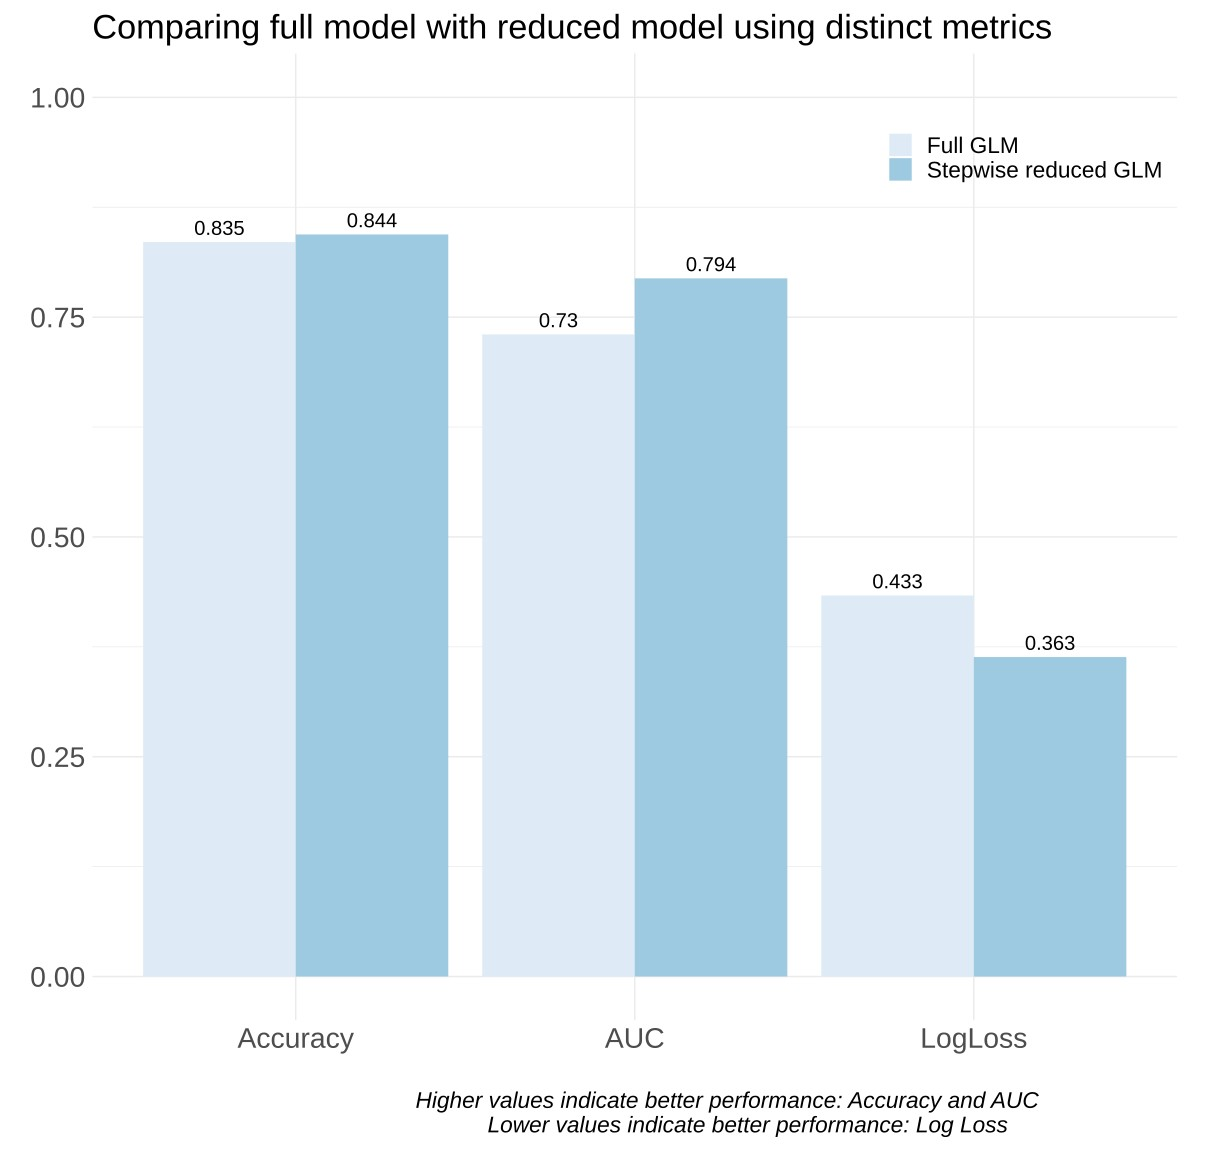
\includegraphics[width=.84\textwidth]{fig4.model.comparison.v1.0.jpg}
\caption{Comparison of the models. The full model including all 32 predictors was compatred in terms of accuracy to the reduced model resulting from the stepwise \textsc{GLM} regression. Values between both models are comparable although only 7 predictors remained in the model compared to the full model. For further details of the multilevel regression cf. Table \ref{tab2:reduced_model}}
\label{fig4:comparison_models}
\end{figure}


\end{document}

